\documentclass[14pt]{matmex-diploma}
\usepackage{xcolor}
\usepackage{hyperref}	
\usepackage{enumitem}
\setlist{nolistsep}
\definecolor{urlcolor}{HTML}{0e0b61}

\hypersetup{
    colorlinks=true,
    linkcolor=black,
    filecolor=magenta,      
    urlcolor=urlcolor,
    pdftitle={Sharelatex Example},
    bookmarks=true,
    pdfpagemode=FullScreen,
}

\begin{document}
\filltitle{ru}{
    chair              = {Направление Математическое обеспечение и администрирование информационных систем},
    title              = {Классификация текстового контента},
    type               = {coursework},
    position           = {студентов},
    group              = 241,
    author             = {Жилкин Федор Игоревич и Смирнов Александр Львович},
    supervisorPosition = {д.\,ф.-м.\,н., профессор},
    supervisor         = {Литвинов Ю.\,В.},
    reviewerPosition   = {д.\,ф.-м.\,н., профессор},
    reviewer           = {Брыксин Т.\,А.},
}
\filltitle{en}{
    chair              = {Software and Administration of Information Systems},
    title              = {Classification of text content},
    type               = {coursework},
    author             = {Fedor Zhilkin and Alexander Smirnov},
    supervisorPosition = {Associate Professor},
    supervisor         = {Yurii Litvinov},
    reviewerPosition   = {professor},
    reviewer           = {Timofey Bryksin},
}
\maketitle
\tableofcontents

\section*{Введение} 

    Для изучения данной работы требуются знания предметной области, поэтому введем некоторые понятия и определения.
    
    \paragraph{Понятия:}
        \begin{itemize}
            \item Бинарная классификация контента — разделение контента на 2 условные группы
            \item Датасет — набор данных
            \item Библиотека классов определяет типы и методы, которые могут быть вызваны из любого приложения
            \item Расширение браузера — компьютерная программа, которая в некотором роде расширяет функциональные возможности браузера
            \item Сервер — локальный компьютер, выполняющий обработку запросов 
            \item GET-запрос запрашивает данные с сервера
            \item POST-запрос  отправляет данные, подлежащие обработке, на указанный сервер
            \item Нейронная сеть - алгоритм машинного обучения, построенный по принципу организации и функционирования биологических нейронных сетей \cite{wiki:nn}
        \end{itemize}
        
    \paragraph{Подходы к классификации текста:}
        \begin{itemize}
            \item Rule-based - подход, основанный на классификации по заданным заранее правилам. Например, по наличию или отсутсвию тех или иных слов
            \item Machine Learning (ML) based - подход, основанный на алгоритмах машинного обучения \cite{wiki:ml}
            \item Hybrid Systems - подход, совмещающий в себе ML Based и Rule-based подходы
        \end{itemize}
        
    \paragraph{Характеристики сравнения эффективности:}    
        \begin{itemize}
            \item Accuracy — общая точность классификатора
            \item Recall — отношение заблокированных взрослых сайтов к общему количеству взрослых сайтов (\% классифицированных взрослых сайтов)
            \item Precision — отношение заблокированных взрослых сайтов к числу всех заблокиронных сайтов (точность блокировки)
            \item F1 Score — среднее гармоническое между Precision и Recall, для учёта и того, и другого в одной величине
        \end{itemize}
    
    \paragraph{Актуальность работы} $\newline$ 
    
        Каждый родитель желает оградить своего ребенка от плохого влияния внешнего мира. Интернет несет в себе не только массу полезной 
        информации, но и огромное количество негатива, которое может сформировать у ребенка неправильное мировоззрение или восприятие
        действительности. Существует еще масса «взрослых» сайтов, просмотр которых ребенку категорически запрещен. Поэтому у родителей 
        возникает вопрос: «Как защитить ребенка от ненужных сайтов?» 
        \begin{figure}[h]
            \centering
            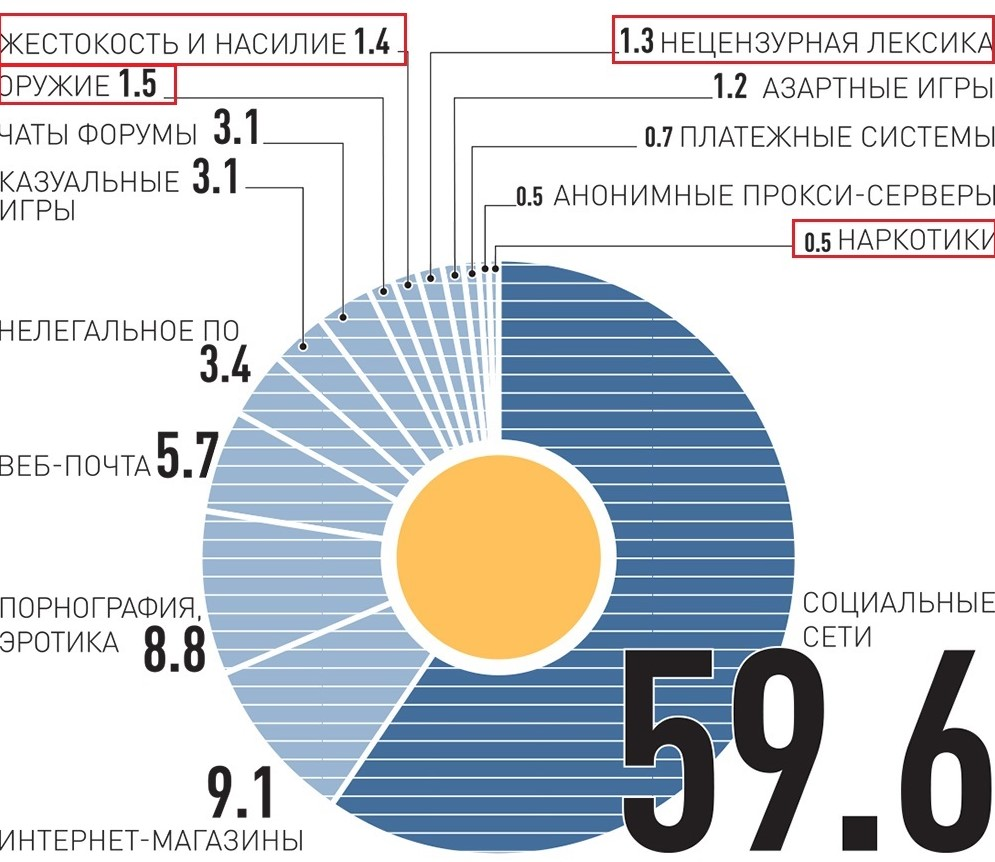
\includegraphics[scale=1.1]{images/children_statistics.jpg}
            \caption{Что интересует детей в интернете (Ист. – Лаборатория Касперского)}
        \end{figure}
        $\newline$ 
    
    \paragraph{Цели} 
        \begin{itemize}
            \item Ограничить детей от взрослого текстового контента в интернете
            \item Получить опыт
            \begin{itemize}
                \item Бинарная классификация текста
                \item Сбор данных для обучения
                \item Написание Python-библиотеки
                \item Написание расширения для Chrome
                \item Написание Python-сервера для приёма запросов
            \end{itemize}
        \end{itemize}
    
    \paragraph{Задачи}
        \begin{itemize}
            \item Провести анализ возможных решений для классификации текста
            \item Собрать рассказы для взрослых и обычные рассказы
            \item Написать Python-сервер, использующий обученную модель для ответа на запросы от расширения
            \item Сделать расширение для Chrome, обращающееся к серверу
        \end{itemize}
    $\newline$ 
    
    Реализация данных задач позволит полностью ограничить детей от негативного влияния интернета, так как программа будет 
    блокировать конкретные страницы, содержащие недопустимый для детей контент.

\section{Обзор существующих решений}

    Существует два типа решения поставленной задачи:
    
    \begin{itemize}
    	\item Ограничения на поиск
    	    \begin{itemize}
    			\item Семейный поиск Яндекс
    	    	\item Безопасный поиск Google
    		\end{itemize}
    	\item Контентная фильтрация
    	    \begin{itemize}
    	    	\item Traffic Inspector
    	    	\item Интернет Цензор
    	    \end{itemize}
    \end{itemize}
    
    Данные решения проблемы не являются оптимальными. В случае ограничения на поиск фильтрация происходит по ключевым словам, 
    что позволяет просматривать непристойный для детей контент, переходя напрямую по ссылкам. 
    Обратная же ситуация с контентной фильтрацией - ограничение накладывается конкретно на определенные ссылки. 
    К тому же большинство таких программ имеют абсолютно не дружелюный интерфейс, не понятный обычному пользователю (\ref{bad}).
    
    \begin{figure}[h]
        \centering
    	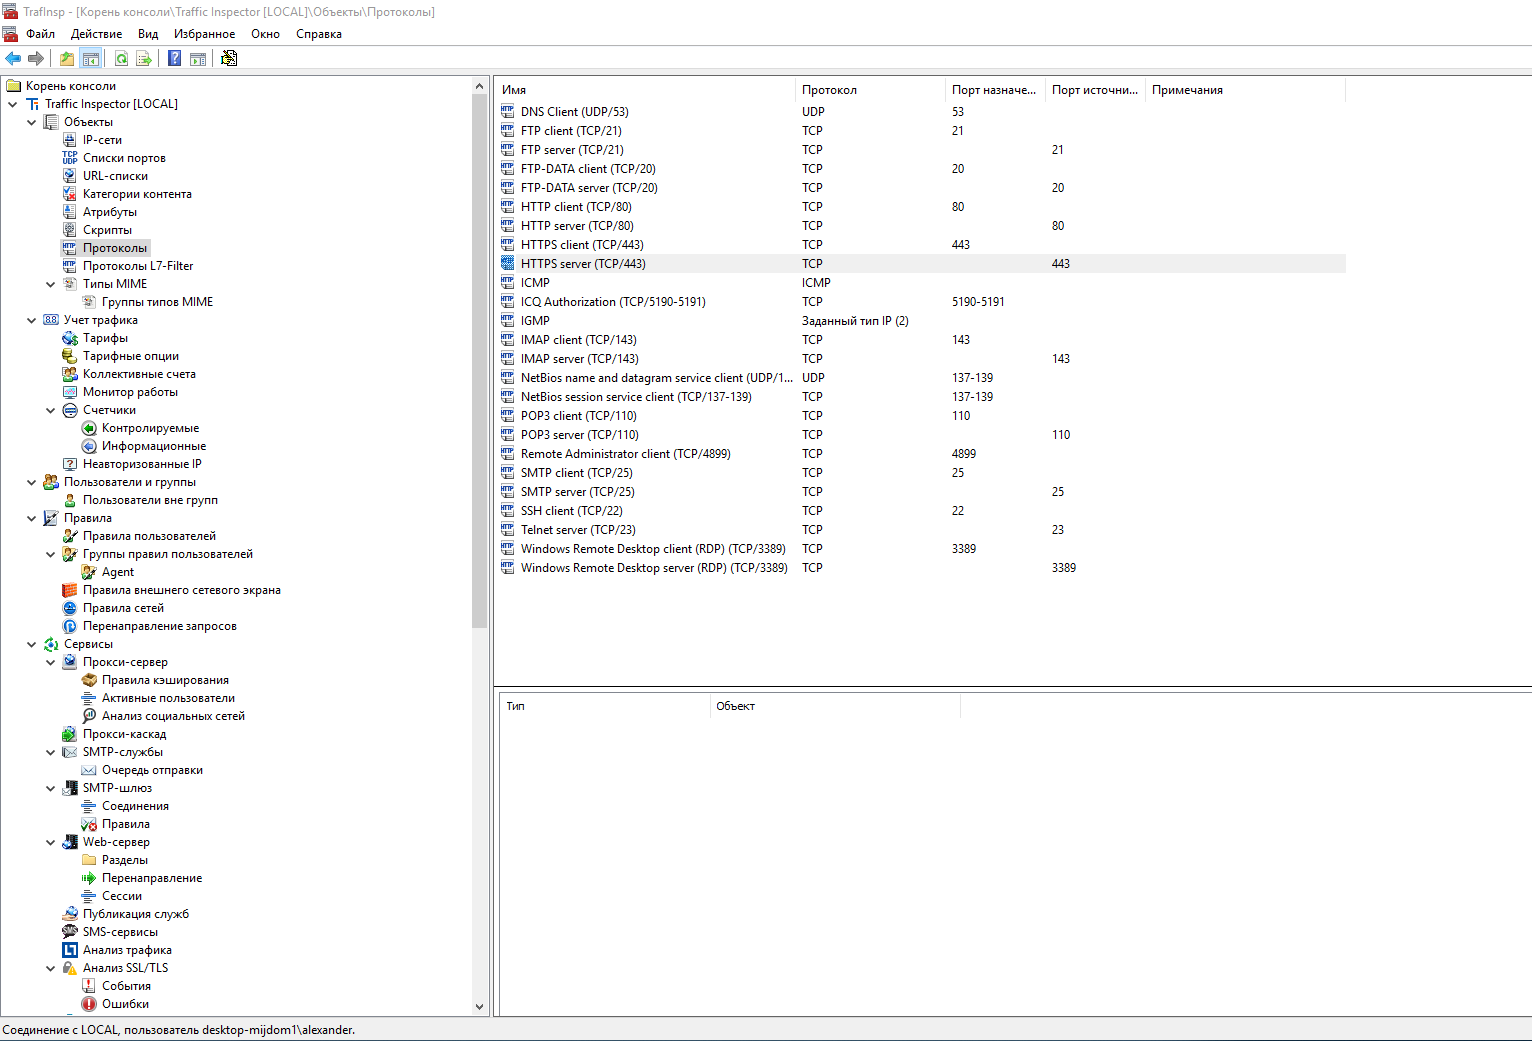
\includegraphics[scale=0.4]{images/bad_interface.png}
    	\caption{Интерфейс программы Traffic Inspector}
    	\label{bad}
    \end{figure}

\section{Описание предлагаемого решения}

    Подход, предлагаемый в данной работе, заключается в том, чтобы классифицировать страницы на взрослые и детские в зависимости
    от текстового контента на них.
    
    Подход классификации веб-страниц по содержимому хорош тем, что в отличие от подходов, основанных на блокировке по URL,
    нам не нужно иметь огромную базу адресов, подлежащих блокировке, которую, к тому же, нужно постоянно поддерживать в актуальном
    состоянии. Также, данный подход имеет преимущество над блокировкой результатов в поисковой выдаче в том, что невозможно будет 
    напрямую попасть на страницу, зная её домен.
    
    Будем применять метод машинного обучения – нейронные сети. Для этого нам нужно
    подготовить данные для обучения, построить модель, обучить модель на размеченных данных и использовать 
    обученную модель для классификации содержимого сайта.
    
    \subsection{Сбор данных} 
    
        Задача сбора данных состоит в том, чтобы собрать большое количество рассказов, подходящих
        только для просмотра людьми, чей возраст выше 18-ти лет, и рассказов, подходящих для чтения 
        людьми всех возрастов.
        
        Рассказы для взрослых будем собирать с сайта ideer.ru с категорий для взрослых. Данный контент отлично подходит,
        так как он содержит в себе как нецензурную лексику, так и слова, используемые только взрослыми людьми.
        Рассказы для широкого круга читалей берём с множества сайтов по разным тематикам.
    
    \subsection{Обучение модели}
    
        Для начала нам необходимо научиться представлять рассказы в виде, в котором мы можем их обрабатывать.
        Делать это мы будем с помощью словаря наиболее популярных в русском языке слов следующим образом:
        каждому рассказу в предложении мы будем сопоставлять список из 10000 элементов (размер словаря), 
        в котором каждым элементом будет являться значение 1 либо 0 (в зависимости от наличия или отсутствия данного слова в словаре).
        Далее мы попробуем и сравним 4 архитектуры:
        
        \begin{itemize}
        	\item Random model – случайный выбор блокировать/не блокировать
        	\item Rule-based model – блокировка по списку непотребных слов
        	\item Classifier – 3-х слойная обычная сеть
        	\item Upgraded Classifier – Classifier, из словаря которой были исключены самые частые слова и добавлена ненормативная лексика
        \end{itemize}
        
        Получили следующие результаты:
        
        \begin{table}[h]
            \begin{tabular}{|l|l|c|c|c|}
            \hline
                                         & F1 Score      & Accuracy & Recall & Precision \\ \hline
            Random model                 & –             & 0.51     & –      & –         \\ \hline
            Rule-based model             & 0.06          & 0.41     & 0.03   & 1.0       \\ \hline
            Classifier                   & 0.90          & 0.88     & 0.93   & 0.87      \\ \hline
            \textbf{Upgraded Classifier} & \textbf{0.91} & 0.90     & 0.92   & 0.91      \\ \hline
            \end{tabular}
        \end{table}
        
        Можем видеть, что наиболее выгодной моделью, как и можно было предположить, является Upgraded Classifier, 
        которую мы и будем использовать в дальнейшем.
        
        Также взглянем на рисунки (\ref{acc}) и (\ref{loss}):
        
        \begin{figure}[!htb]
           \begin{minipage}{0.48\textwidth}
             \centering
             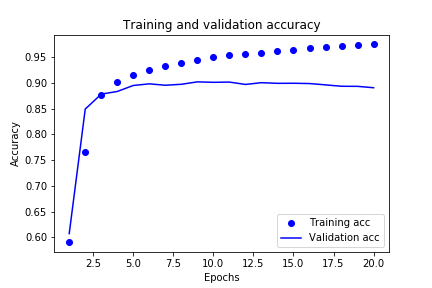
\includegraphics[width=.9\linewidth]{images/acc.png}
             \caption{Зависимость точности от количества эпох}\label{acc}
           \end{minipage}\hfill
           \begin{minipage}{0.48\textwidth}
             \centering
             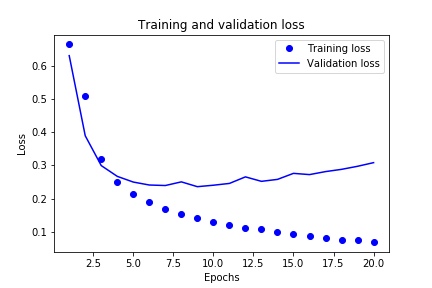
\includegraphics[width=.9\linewidth]{images/loss.png}
             \caption{Зависимость потерь от количества эпох}\label{loss}
           \end{minipage}
        \end{figure}
        
        Из зависимости на (\ref{acc}) можно сделать вывод, что после 10-ти эпох точность предсказаний модели на данных, которых
        она ещё не видела, не растёт, вследствие чего дальнейшее обучение не имеет смысла. На (\ref{loss}) видно, что после 7-й 
        итерации обучения функция потерь начинает расти, что свидетельствует о переобучении модели и необходимости 
        преостановить обучение.

    
    \subsection{Расширение для Chrome и сервер}
    
        Следующим шагом явлется написание сервера, задача которого обрабатывать POST/GET запросы от расширения. Работает он следующим образом:
        Получаем POST-запрос от расширения с текущей html-страницей, выбираем из него все русские слова, классифицируем страницу по заранее обученной
        модели и записываем результат в файл. Далее мы получаем GET-запрос и отправляем расширению полученный результат из файла (\ref{uml}).
    
        Работает это следующим образом:
        \begin{figure}[h]
            \centering
        	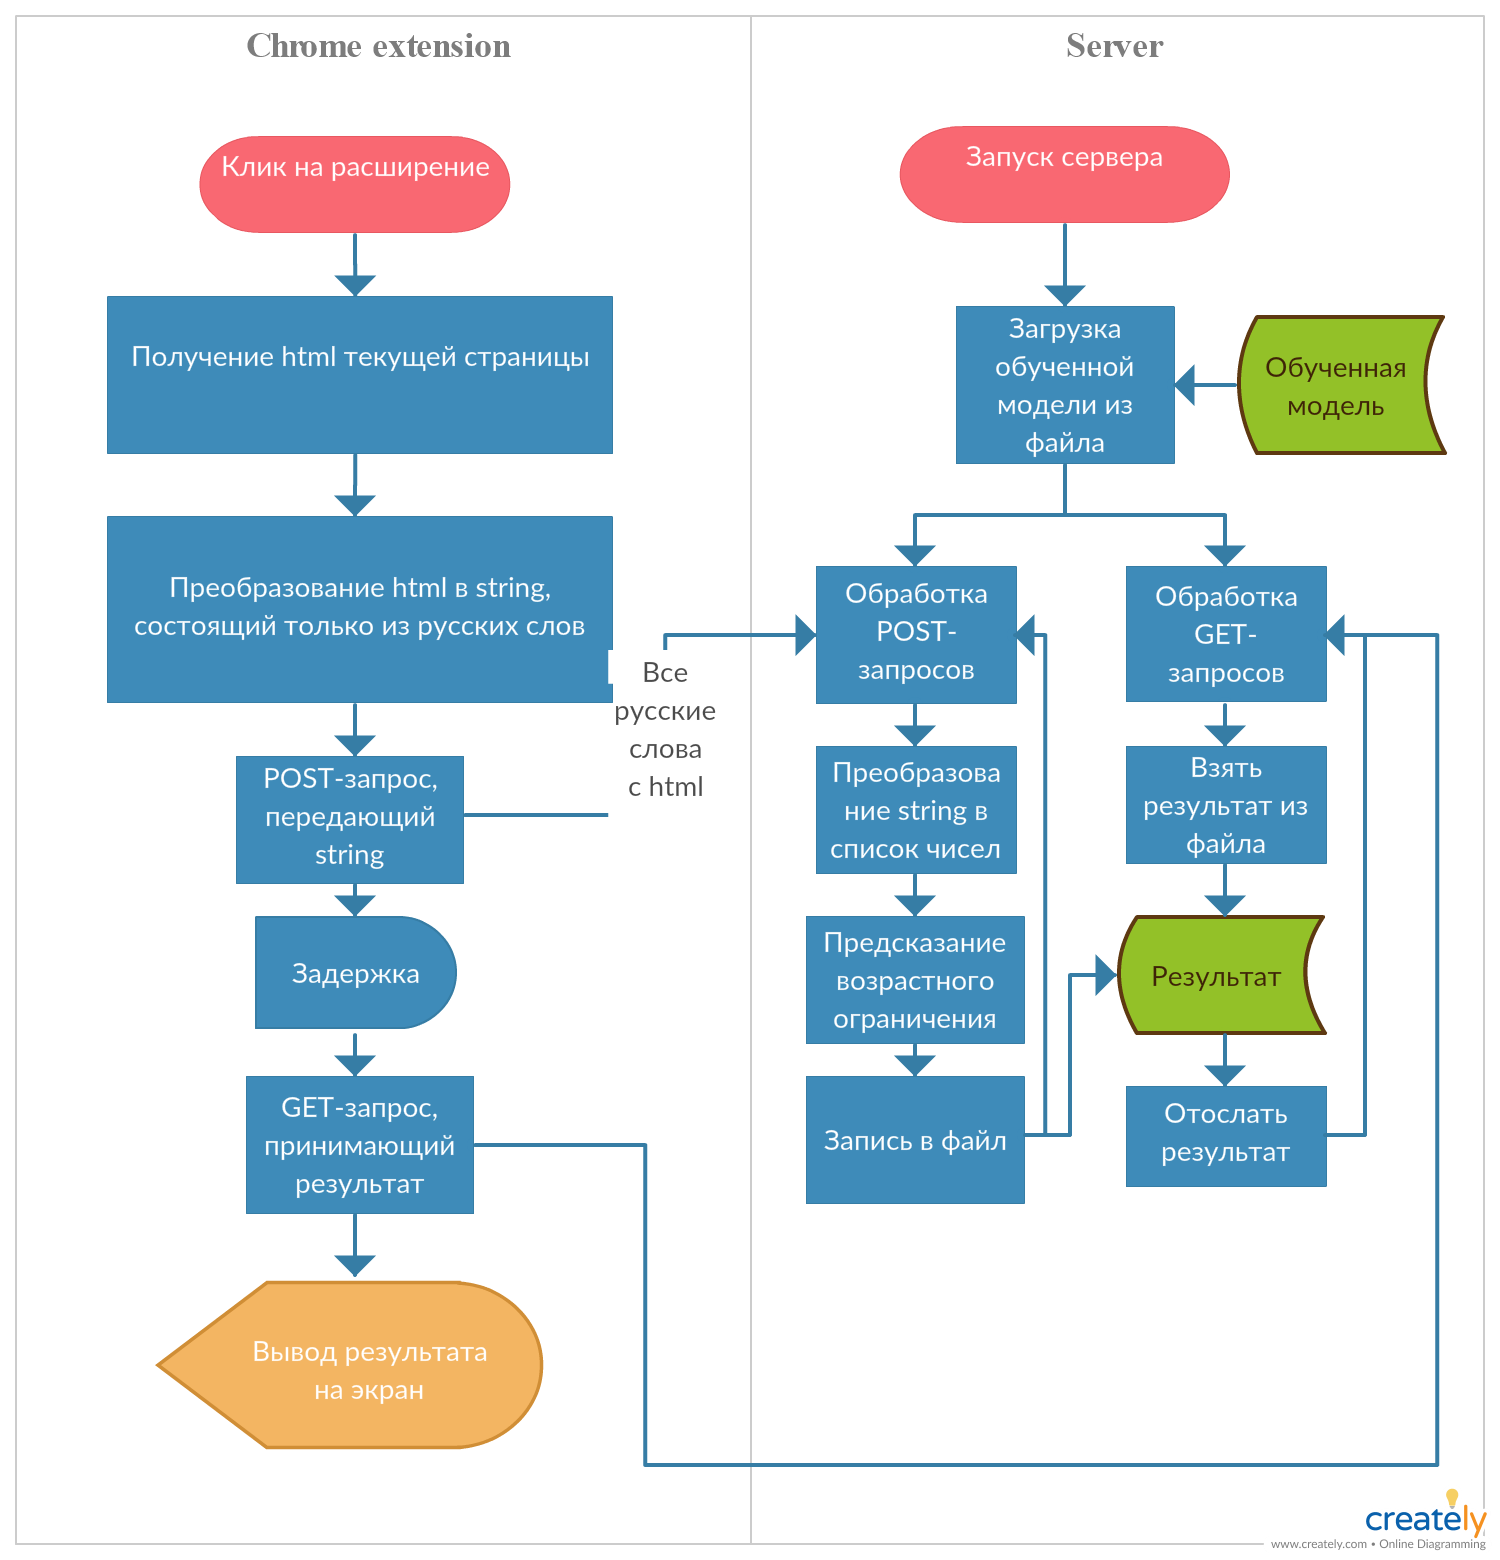
\includegraphics[scale=0.22]{images/uml.png}
        	\caption{Диаграмма взаимодействия расширения и сервера}
        	\label{uml}
        \end{figure}     
        
\section*{Заключение}        
    \begin{Large}
            \begin{itemize}
                \item \href{https://github.com/SmirnovAlexander/PoemClassifier}{Сделано расширение для Chrome}
                \item \href{https://pypi.org/project/TalesParse/}{Сделана библиотека на pypi} 
                \item \href{https://www.kaggle.com/idoldev/adult-and-child-russian-tales-dataset-with-label}{Собраны рассказы на kaggle}  
                \item \href{https://github.com/Feodoros/Scraping_Tales}{Написан сборщик рассказов}
            \end{itemize}
    \end{Large}

\setmonofont[Mapping=tex-text]{CMU Typewriter Text}
\bibliographystyle{ugost2008ls}
\bibliography{diploma.bib}
\end{document}